\begin{figure}[t!]
\centering
  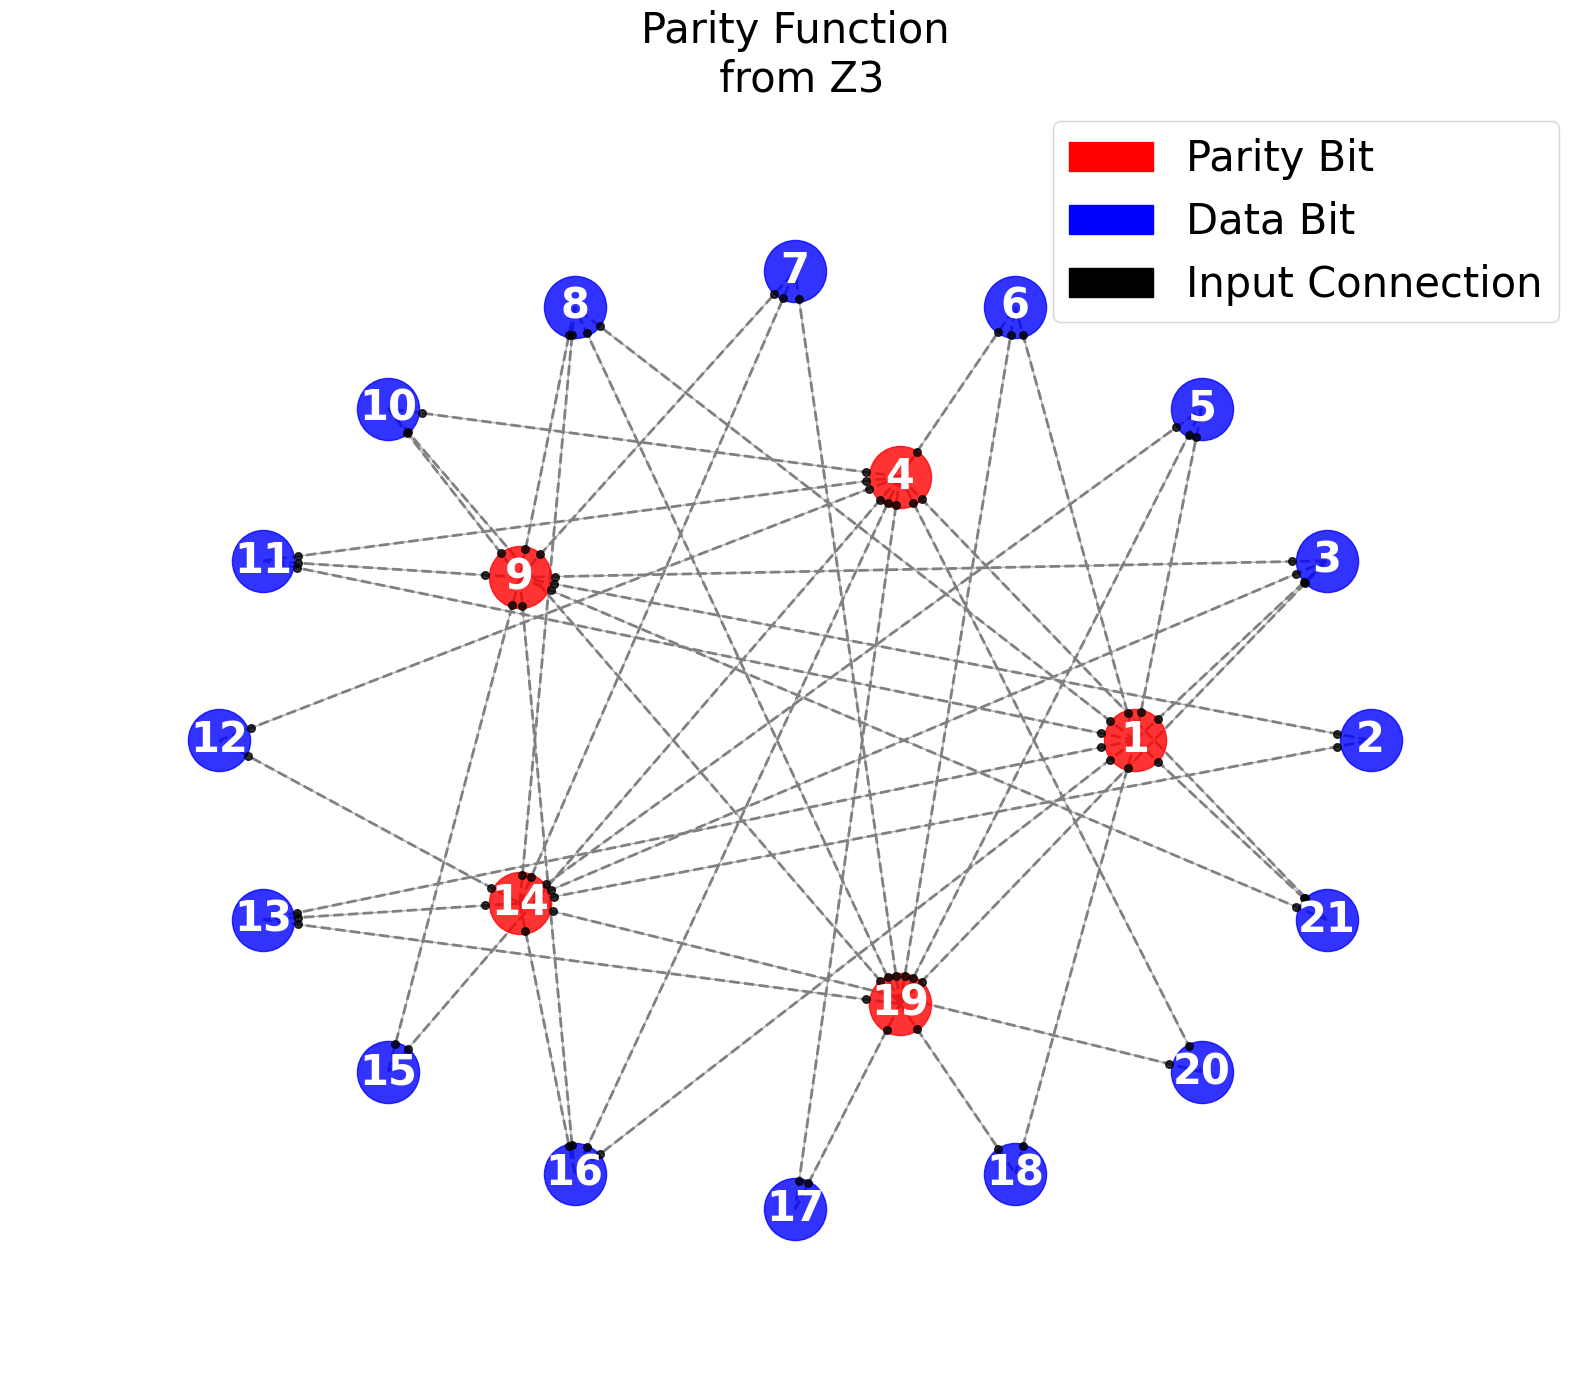
\includegraphics[width=0.9\linewidth]{img/parity.png}
  \caption{Parity function reverse engineered from \cite{tay2023afm}. After modeling as a Z3 SAT problem, exactly one satisfiable parity matrix is returned. Each parity bit is an XOR of 9 input bits. The $d_{min}$ of this code is 2, indicating that this code is not a standard linear block code.}
\label{fig:oxram-parity-func}
\end{figure} 